\subsection{Diagramme de d\'{e}ploiement}


\begin{itemize}
\item{ \textbf{Le Client :} C'est le navigateur web, il permet aux utilisateurs d'acc\'{e}der au
serveur, c'est d'interface \`{a} l'utilisateur.}

\item{ \textbf{Le serveur web :} C'est le serveur principal qui abrite les diff\'{e}rents composants logiciels de
notre application. Il assure la gestion des connexions et des requ\^{e}tes du client
ainsi que aussi la distribution et rendu (rendering) des pages EJS.
Cet \'{e}l\'{e}ment contient principalement un environnement d'ex\'{e}cution qui est
le framework javascript Node js sur lequel est d\'{e}ploy\'{e} l'application
Web(Express JS ).}

\item{ \textbf{La base de donn\'{e}es :} Est exploit\'{e} par le avec le serveur wamp.
C'est le composant qui s'occupe du stockage et de la gestion des donn\'{e}es.
La communication des donn\'{e}es entre l'application est la base de donn\'{e}es
est assur\'{e}e par le pilote ( driver ) de mysql pour Node js.}


\end{itemize}





\begin{figure}[H]
\center
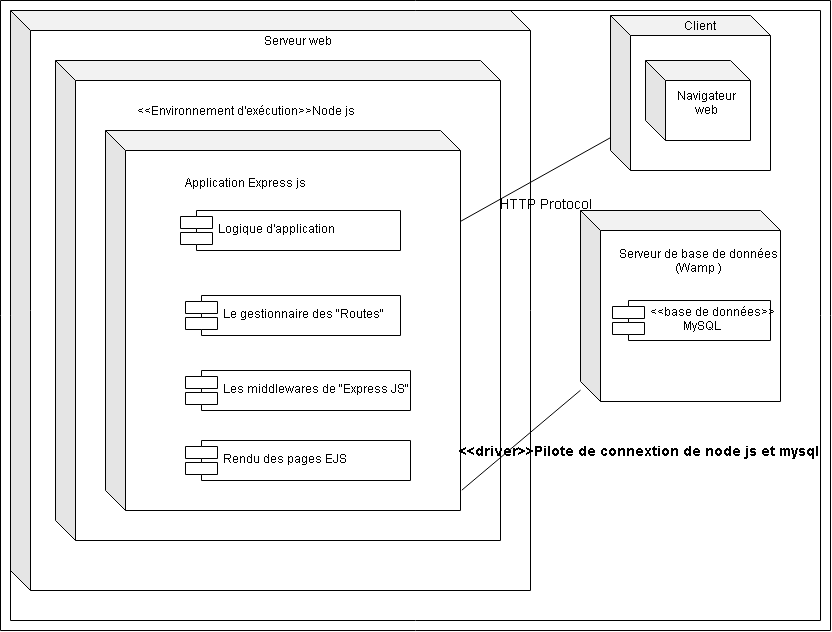
\includegraphics[width=13cm,height=11cm]{./figures/deployement.png}
\caption{Diagramme de d\'{e}ploiement.}
\end{figure}
\FloatBarrier
